\chapter{Programmierung}
\section{Attribute Fahrzeug}
\textbf{Schwierigkeit:} Welche Eigenschaften müssen einem Auto übergeben werden damit eine realistische Simulation möglich ist?
\begin{addmargin}[25pt]{0pt}
	\item \textbf{Lösungsansatz:} Beim Erstellen erhält das Auto eine Position und eine Geschwindigkeit. Die Position besteht aus einer Meteranzeige, wo auf der Strecke es sich aufhält und einer Abfrage auf welcher Spur es sich befindet. Zudem hat es die Möglichkeit zu beschleunigen bezeihungsweise zu bremsen und kann die zugelassene Höchstgeschwindigkeit abfragen. Die Länge jedes Fahrzeugs beträgt 4,5\,m. Das bedeutet, dass LKWs in der Simulation nicht betrachtet werden.\\
\end{addmargin}

\section{Visualisierung}
\textbf{Schwierigkeit:} Wie lässt sich das Reißverschlussverfahren am besten simulieren?
\begin{addmargin}[25pt]{0pt}
	\item \textbf{Lösungsansatz:} Für die Simulation wurde Slick verwendet, da alle Gruppenmitglieder schon Erfahrungen mit Java gesammelt haben und Slick bereits eine graphische Oberfläche für Java besitzt, auf die zugegriffen werden konnte. Somit konnte gleich mit der Implementierung des Reißverschlussverfahrens begonnen werden und es musste nicht erst eine graphische Umgebung erstellt werden. Um einen leichteren Einstieg in Slick zu erhalten,wurde ein bereits existierendes Spiel namens "'UfoInvasion"' benutzt, um zu überprüfen, ob Slick auf allen Computern läuft. Daraufhin wurde ein neues Programm geschrieben, in dem lediglich die Slick-Library übernommen wurde. \\
\end{addmargin}
\textbf{Schwierigkeit:} Wie sollte die Fahrbahn aufgebaut sein?
\begin{addmargin}[25pt]{0pt}
	\item \textbf{Lösungsansatz:} Betrachtet wird eine Fahrbahnlänge von 1200\,m. Die Länge wurde gewählt, da sie lang genug ist, um die Auswirkungen des Reißverschlussverfahrens zu beurteilen, zugleich aber nicht zu groß, damit die einzelnen Autos noch erkennbar sind. Um einen kleinerer Abschnitt zu betrachten, gibt es auch die Möglichkeit heranzuzoomen.\\
\end{addmargin}
\textbf{Schwierigkeit:} Was für visuelle Eigenschaften muss das Auto besitzen?
\begin{addmargin}[25pt]{0pt}
	\item \textbf{Lösungsansatz:} Um die Handlung jedes einzelne Auto zu erkennen, haben wir den Autos Bremslichter und Blinker gegeben. Damit man diese Aktionen auch bei sehr klein abgebildeten Fahrzeugen erkennbar ist, blinkt außerdem die Umrandung. Zudem zeigt die Fahrzeugfarbe den Fahrstyle an. Der aggressive Fahrer ist durch rosa, der neutrale durch blau und der passive durch grün gekennzeichnet.\\
\end{addmargin}

\begin{figure} %Abbildung Fahrzeugtypen: Aggressiv, Neutral, Passiv
\begin{subfigure}{0.1\linewidth}
		\centering
		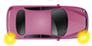
\includegraphics[width=\linewidth]{images/indicating_a}
		\label{fig:indicatinga}
\end{subfigure}
\begin{subfigure}{0.11\linewidth}
	\centering
	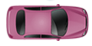
\includegraphics[width=\linewidth]{images/normal_a}
	\caption*{Aggressiv}
	\label{fig:normala}
\end{subfigure} 
\begin{subfigure}{0.1\linewidth}
		 \centering
		 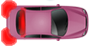
\includegraphics[width=\linewidth]{images/breaking_a}
		 \label{fig:breakinga}
\end{subfigure} 
\begin{subfigure}{0.1\linewidth}
		\centering
		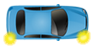
\includegraphics[width=\linewidth]{images/indicating_n}
		\label{fig:indicatingn}
\end{subfigure} 
\begin{subfigure}{0.11\linewidth}
	\centering
	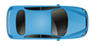
\includegraphics[width=\linewidth]{images/normal_n}
	\caption*{Neutral}
	\label{fig:normaln}
\end{subfigure} 
\begin{subfigure}{0.1\linewidth}
	\centering
	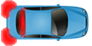
\includegraphics[width=\linewidth]{images/breaking_n}
	\label{fig:breakingn}
\end{subfigure} 
\begin{subfigure}{0.1\linewidth}
\centering
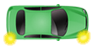
\includegraphics[width=\linewidth]{images/indicating_p}
\label{fig:indicatingp}
\end{subfigure}  
\begin{subfigure}{0.11\linewidth}
			\centering
			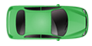
\includegraphics[width=\linewidth]{images/normal_p}
			\caption*{Passiv}
			\label{fig:normalp}
\end{subfigure} 
\begin{subfigure}{0.1\linewidth}
	\centering
	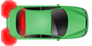
\includegraphics[width=\linewidth]{images/breaking_p}
	\label{fig:breakingp}
\end{subfigure}
\caption{Fahrzeugtypen: Aggressiv, Neutral, Passiv}
\label{fig:fahrzeug}
\end{figure}

\section{Spawner}
\textbf{Schwierigkeit:} Wie schafft man es einen realistischen Verkehrsfluss zu erzeugen, um den Eingangsverkehr in das Simulationsgebiet zu Simulieren.
%Wie schafft man es Fahrzeuge zu erzeugen, die mit einem realistischen Verkehrsverhalten an das Stauende fahren.
\begin{addmargin}[25pt]{0pt}
	\item \textbf{Lösungsansatz:} Da die Simulation lediglich ein beschränktes Gebiet betrachtet, ist es notwendig, dass in das Gebiet hineinfließende Verkehrsverhalten möglichst realistisch darzustellen. Hierbei beschr\"ankt sich das Modell auf folgende Aspekte: 
\begin{itemize}
	\item Der Sicherheitsabstand wird eingehalten.
	\item Fahrzeuge werden mit ähnlicher Geschwindigkeit erzeugt.
	\item Fahrzeuge fahren links schneller, aufgrund des rechtsseitigen Überholverbots.
	\item Auf der rechten Fahrspur gibt es eine höhere Verkehrsdichte.
\end{itemize}
Um ein neues Fahrzeug in die Simulationsumgebung einzuzufügen, wird eine normal verteilte Zufallszahl gewählt, welche den Zeitpunkt für die Erzeugung eines Autos beschreibt. Erwartungswert und Standardabweichung verhalten sich umgekehrt proportional zur gewünschten Verkehrsdichte. Ist dieser Zeitpunkt erreicht, wird anhand der voraus fahrenden Autos der vorhandene Platz berechnet. Damit ein Auto erzeugt werden kann, muss der vorhandene Platz mindestens den Sicherheitsabstand betragen. Zusätzlich wird die Geschwindigkeitsbeschränkung für das erzeugte Auto berechnet. Diese Geschwindigkeitsbeschränkung ist so definiert, dass das Auto noch genug Zeit zum Bremsen hat, um einen Unfall zu vermeiden. Eine ähnliche Geschwindigkeit wir dadurch gewährleistet, dass die Geschwindigkeit in Abhängigkeit der derzeitigen Verkehrsgeschwindigkeit berechnet wird, jedoch die Geschwindigkeitsbeschränkung nicht überschreiten darf. Zusätzlich müssen Fahrzeuge die auf der linken Spur erzeugt werden mindestens die Spurgeschwindigkeit der rechten Spur besitzen, um das rechtsseitige Überholen zu verhindern.
%TODO Fahrertypen??
\end{addmargin}

\section{Bedienung}
\textbf{Schwierigkeit:} Wie erhält man eine benutzerfreundliche Bedienungsoberfläche, bei der man möglichst viele Variablen verändern kann.
\begin{addmargin}[25pt]{0pt}
	\begin{figure}
		\begin{subfigure}{0.5\linewidth}
			\centering
			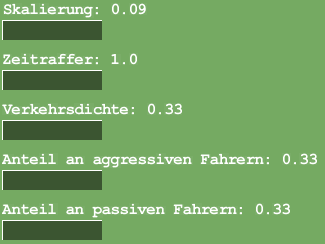
\includegraphics[width=\linewidth]{images/Eingabe}
			\caption*{Eingabefelder}
			\label{fig:eingabe}
		\end{subfigure}
		\begin{subfigure}{0.5\linewidth}
			\centering
			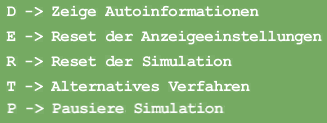
\includegraphics[width=\linewidth]{images/Bedienung}
			\caption*{Shortcuts}
			\label{fig:shortcuts}
		\end{subfigure}
	\caption{Bedienelemente}
	\label{fig:bedienung}
	\end{figure}
	
	\item \textbf{Lösungsansatz:} Die Steuerung über Eingabefelder (Abb.\ref{fig:bedienung}) hat sich als am benutzerfreundlichsten herausgestellt. Hier hat der Benutzer die Möglichkeit auf Skalierung, Zeitraffer, Verkehrsdichte, sowie den Anteil der Fahrertypen Einfluss zu nehmen. Um Fehler zu vermeiden, werden nur sinnvolle Eingaben berücksichtig.\\ 
Mithilfe der Skalierung kann man an die Verengung heranzoomen. Bei der Standardeinstellung von 0.09 wird der komplette Simulationsbereich betrachten.\\ 
Der Zeitraffer dient dazu Langzeitentwicklungen schneller darstellen zu können. Hierbei ist jedoch zu beachten, dass durch die Verwendung des Zeitraffers die Abtastrate sinkt. Dadurch kann es zu Genauigkeitsverlusten kommen. Bis zur fünffachen Geschwindigkeit sind die Ergebnisse noch relativ genau, bei einer schnelleren Betrachtung dient das Ergebnis lediglich als grobe Annäherung.\\
Durch die Verkehrsdichte kann man die Erzeugungswahrscheinlichkeit von Fahrzeugen verändern. Die Verkehrsdichte hat massgeblichen Einfluss auf die Effektivität des Reißverschlussverfahrens. Diesen Einfluss kann der Benutzer anhand der ausgegebenen Durchschnittsgeschwindigkeit, der Eingangsverkehrsdichte, sowie der Ausgangsverkehrsdichte ablesen.\\
Zu guter letzt kann der Benutzer noch den Anteil der Fahrertypen variieren. Standardmäßig gibt es 33\% aggressive (rosa), 33\% passive (grün) und 33\% neutrale Fahrer (blau). Die Anteile addieren sich immer zu 100\% auf, wobei die aggressiven und passiven Anteile durch Eingabefelder veränderbar sind und der neutrale Fahrer die restlichen Anteile bekommt.\\\\
	Zusätzlich wurden mehrere Shortcuts (Abb. \ref{fig:bedienung}) implementiert:
	\begin{itemize}
		\item \textbf{Verfahren wechseln}\\
		Mithilfe von "'T"' lässt sich das Reißverschlussverfahren wechseln. Hierbei wird zusätzlich ein Reset ausgeführt.
		\item \textbf{Fahrzeugdaten anzeigen}\\
		Solle der Benutzer zusätzliche Informationen zu den jeweiligen Autos bekommen wollen, kann er durch Betätigung des "'D"' auf der Tastertur sich zu jedem Auto dessen ID, die derzeitige Geschwindigkeit, sowie die Beschleunigung anzeigen lassen. Diese Funktion wurde zum Debuggen erstellt, wodurch kein großer Wert auf die Lesbarkeit gelegt wurde und somit sich die Datenausgaben überlagern können.
		\item \textbf{Reset}\\
		Mithilfe von "'R"' kann man die Simulation reseten. Dabei werden alle Fahrzeuge entfernt.\\
		Wird "'E"' gedrückt werden alle getroffenen Einstellungen wieder auf die Standardeinstellung gesetzt.
		\item \textbf{Pause}\\
		"'P"' pausiert und setzt die Simulation fort.
	\end{itemize}
\end{addmargin}

\section{Fahrer}
\textbf{Schwierigkeit:} Es gibt in der Realität viele unterschiedliche Fahrertype. Jeder Fahrer hat einen individuellen Fahrstyle. Diese lassen sich häufig in Kategorien wie zum Beispiel aggressive oder passive Fahrer einordnen. Ganz ohne die Unterscheidung von Fahrertypen wäre die Simulation nicht Realitätsgetreu.
\begin{addmargin}[25pt]{0pt}
	\item \textbf{Lösungsansatz:} Die Programmierung von sehr vielen Fahrertypen ist zeitaufwendig und alle psychologischen Aspekte sind nicht darstellbar. Es wurden drei Fahrertypen implementiert: Der Aggressiven (rosa), der Neutralen (blau) und der Passiven (grün). Diese drei Fahrertypen unterscheiden sich darin, wie großen Sicherheitsabstand sie einhalten, mit welcher Geschwindigkeit sie erzeugt werden, wie stark der Fahrer abbremst sobald das vorausfahrende Fahrzeug bremst und wie sie sich beim Einsortieren verhalten. So hat der aggressive Fahrer eine deutlich höhere Wahrscheinlichkeit, dass er mit einer erhöhten Geschwindigkeit erzeugt wird, als der passive oder neutrale Fahrer. Zudem nutzt der aggressive Fahrer jede noch so kleine Lücke die sich bei der Verengung ergibt. Der Passive hingegen lässt einen deutlich größerenen Sicherheitsabstand zum vorausfahrenden Fahrzeug und hat einen höheren "Panikfaktor", welcher bewirkt, dass er sobald vorne gebremst wird, auch stark abbremst.\\
Um die Simulation realitätsgetreuer zu machen besitzt jeder Fahrer eine Reaktionszeit von 250\,ms. Dadurch bremsen nicht alle Fahrzeuge gleichzeitig sondern erst wenn der Vordermann auch bremst.\\
\end{addmargin}